%!TEX root=../ast2016.tex

\section{Empirical Study}
\label{sec:empirical-study}

\subsection{Experimental Setup}

%!TEX root=../ast2016.tex

\begin{table}[t!]
	\caption{Schemas analysed in the empirical study} \label{tbl:study-schemas}
	\scriptsize
	\centering
	\scalebox{\tablescalefactor}{
		\begin{tabular}{l@{\hskip -5pt}rrrrrrrr}
			{Schema}           & \rot{Tables} & \rot{Columns} & \rot{Checks} & \rot{Foreign Keys} & \rot{Not Nulls} & \rot{Primary Keys} & \rot{Uniques} & \rot{$\sum$Constraints} \\ \hline
			ArtistSimilarity & 2 & 3 & 0 & 2 & 0 & 1 & 0 & 3 \\
			ArtistTerm & 5 & 7 & 0 & 4 & 0 & 3 & 0 & 7 \\
			BankAccount & 2 & 9 & 0 & 1 & 5 & 2 & 0 & 8 \\
			BookTown & 22 & 67 & 2 & 0 & 15 & 11 & 0 & 28 \\
			BrowserCookies & 2 & 13 & 2 & 1 & 4 & 2 & 1 & 10 \\
			Cloc & 2 & 10 & 0 & 0 & 0 & 0 & 0 & 0 \\
			CoffeeOrders & 5 & 20 & 0 & 4 & 10 & 5 & 0 & 19 \\
			CustomerOrder & 7 & 32 & 1 & 7 & 27 & 7 & 0 & 42 \\
			DellStore & 8 & 52 & 0 & 0 & 39 & 0 & 0 & 39 \\
			Employee & 1 & 7 & 3 & 0 & 0 & 1 & 0 & 4 \\
			Examination & 2 & 21 & 6 & 1 & 0 & 2 & 0 & 9 \\
			Flights & 2 & 13 & 1 & 1 & 6 & 2 & 0 & 10 \\
			FrenchTowns & 3 & 14 & 0 & 2 & 13 & 0 & 9 & 24 \\
			Inventory & 1 & 4 & 0 & 0 & 0 & 1 & 1 & 2 \\
			Iso3166 & 1 & 3 & 0 & 0 & 2 & 1 & 0 & 3 \\
			iTrust & 42 & 309 & 8 & 1 & 88 & 37 & 0 & 134 \\
			JWhoisServer & 6 & 49 & 0 & 0 & 44 & 6 & 0 & 50 \\
			MozillaExtensions & 6 & 51 & 0 & 0 & 0 & 2 & 5 & 7 \\
			MozillaPermissions & 1 & 8 & 0 & 0 & 0 & 1 & 0 & 1 \\
			NistDML181 & 2 & 7 & 0 & 1 & 0 & 1 & 0 & 2 \\
			NistDML182 & 2 & 32 & 0 & 1 & 0 & 1 & 0 & 2 \\
			NistDML183 & 2 & 6 & 0 & 1 & 0 & 0 & 1 & 2 \\
			NistWeather & 2 & 9 & 5 & 1 & 5 & 2 & 0 & 13 \\
			NistXTS748 & 1 & 3 & 1 & 0 & 1 & 0 & 1 & 3 \\
			NistXTS749 & 2 & 7 & 1 & 1 & 3 & 2 & 0 & 7 \\
			Person & 1 & 5 & 1 & 0 & 5 & 1 & 0 & 7 \\
			Products & 3 & 9 & 4 & 2 & 5 & 3 & 0 & 14 \\
			RiskIt & 13 & 57 & 0 & 10 & 15 & 11 & 0 & 36 \\
			StackOverflow & 4 & 43 & 0 & 0 & 5 & 0 & 0 & 5 \\
			StudentResidence & 2 & 6 & 3 & 1 & 2 & 2 & 0 & 8 \\
			UnixUsage & 8 & 32 & 0 & 7 & 10 & 7 & 0 & 24 \\
			Usda & 10 & 67 & 0 & 0 & 31 & 0 & 0 & 31 \\
			\hline
			{Total} & 172 & 975 & 38 & 49 & 335 & 114 & 18 & 554 \\
			\hline

		\end{tabular}
	}
\end{table}


\begin{itemize}
  \item 32 schemas
    \begin{itemize}
      \item 1 to 42 tables
      \item 3 to 309 columns
      \item 0 to 134 constraints
      \item Includes each of the types of constraint supported by \SchemaAnalyst (\PK, \FK, \NOTNULL, \UNIQUE and \CHECK constraints)
    \end{itemize}
  \item 3 DBMSs -- \Postgres, \HyperSQL (in-memory), \SQLite (in-memory)
  \item 30 repeated trials
  \item 2 techniques -- \Original and \VirtualMutationAnalysis
  \item Metrics -- time taken for mutation analysis, number of mutants, number of test cases
  \item Mention that the mutation scores of the Original technique are used to validate the results given by virtual mutation analysis, and that in every case the results were identical. (Possibly repeat this in the threats section?)
\end{itemize}

\paper{Mutation2013}{To perform the experiments, we used the Java programming language to implement our approach in the SchemaAnalyst tool [3]. SchemaAnalyst was compiled with the JDK 7 compiler and executed with the Oracle Java 1.7 64-bit virtual machine for Linux. We executed the experiments on a \_\_\_\_\_\_ machine, \_\_\_\_\_\_ 64-bit kernel, with a \_\_\_\_\_\_ GHz CPU and \_\_\_\_\_\_ RAM. The specific DBMS versions were Postgres \_\_\_\_\_\_ and SQLite \_\_\_\_\_\_, used in \_\_\_\_\_\_ configurations.}\todo{Add version number for HyperSQL. Mention that SQLite and HyperSQL were `in-memory'.}

\subsection{Empirical Results}

\begin{table*}[t]
  \caption{\label{tbl:time_saved_by_dbms_table}
    Time saving summary.
  }\vspace{1em}
  \scriptsize
  \centering
  \scalebox{\tablescalefactor}{
    \begin{tabular}{|l|r|r|r|r|r|r|r|r|}
      \hline
      \multirow{2}{*}{DBMS} & Proportion & \multicolumn{3}{c|}{Time taken (ms)} & \multicolumn{3}{c|}{Time taken (\%)} & \multirow{2}{*}{Total (ms)} \\ \cline{3-8}
                            & \multicolumn{1}{c|}{faster} & Mean & Max & Min & Mean & Max & Min & \\
      \hline
      HyperSQL & 1.00 & 12,499 & 358,707 & 1 & 0.69 & 0.97 & 0.23 & 399,968\\
      \hline
      Postgres & 1.00 & 872,356 & 24,932,544 & 1 & 0.99 & 1.00 & 0.87 & 27,915,395\\
      \hline
      SQLite & 0.84 & 20,174 & 614,607 & -30 & 0.40 & 1.00 & -0.50 & 645,575\\
      \hline
    \end{tabular}
  }
\end{table*}

\subsubsection{Research questions}

\textbf{RQ1: }\emph{How does the time taken by Virtual mutation analysis compare to the Original technique, and how does
this vary depending on the DBMS in use?}\\

\textbf{RQ2: }\emph{Is the performance of Virtual mutation analysis dependant upon (a) the number of test cases being
executed, or (b) the number of mutants being analysed?}\\

\textbf{RQ3: }\emph{(RQ regarding number of mutants that can be analysed in the same time)}\\

\begin{figure*}[t]
  \centering
  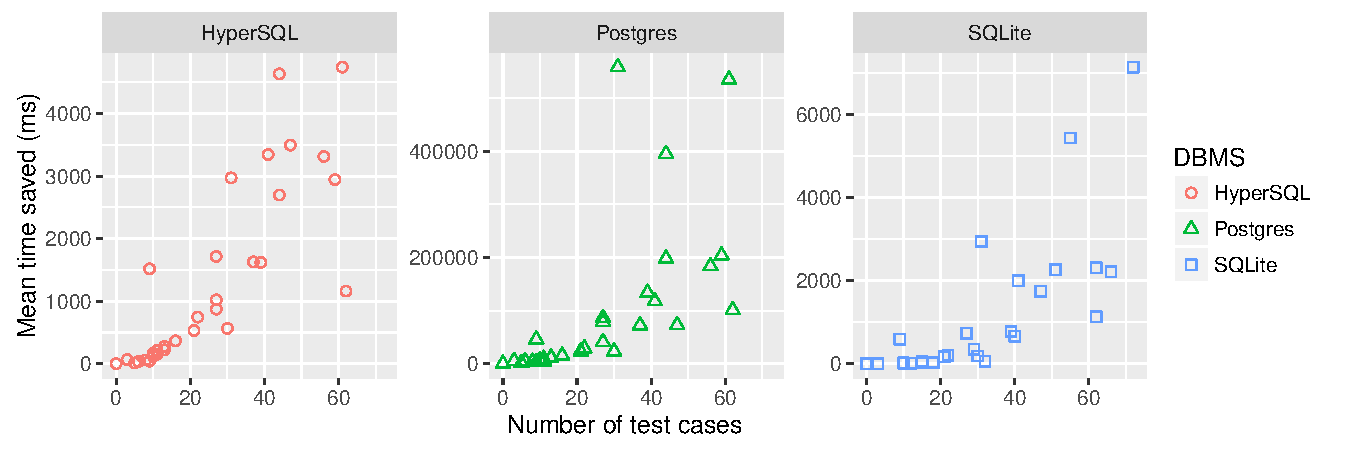
\includegraphics[width=6in]{graphics/time_saved_vs_tests_scatter_noitrust_facetdbms.pdf}
  \caption{Scatter plot of time saved against number of tests.}
  {\small Values for the \texttt{iTrust} schema are excluded to prevent scaling issues but follow a similar trend.}
\end{figure*}

\begin{figure*}[t]
  \centering
  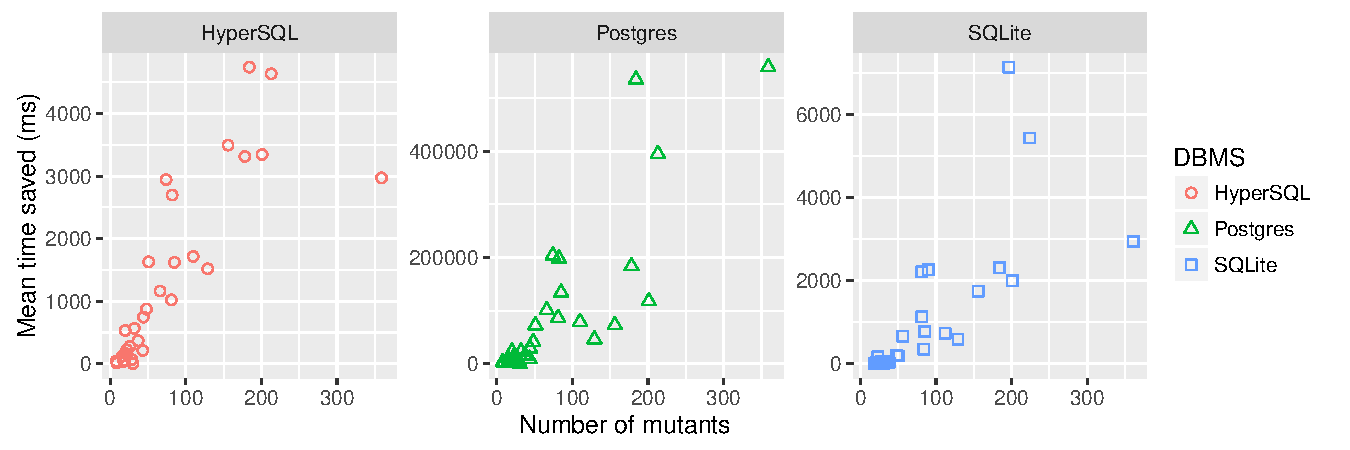
\includegraphics[width=6in]{graphics/time_saved_vs_mutants_scatter_noitrust_facetdbms.pdf}
  \caption{Scatter plot of time saved against number of mutants.}
  {\small Values for the \texttt{iTrust} schema are excluded to prevent scaling issues but follow a similar trend.}
\end{figure*}


\subsection{Threats to Validity}
